\documentclass{beamer}
\usepackage{beamerthemesplit}
\usetheme{SPbGU}
%{CambridgeUS}
% Выпишем часть возможных стилей, некоторые из них могут содержать
% дополнительные опции
% Darmstadt, Ilmenau, CambridgeUS, default, Bergen, Madrid, AnnArbor,Pittsburg, Rochester,
% Antiles, Montpellier, Berkley, Berlin
\usepackage{pdfpages}
\usepackage{amsmath}
\usepackage{cmap} % for serchable pdf's
\usepackage[T2A]{fontenc} 
\usepackage[utf8]{inputenc}
\usepackage[english,russian]{babel}
%\uselanguage{russian}\languagepath{russian}
\usepackage{indentfirst}
\usepackage{amsmath}
\usepackage{array}
%\usepackage{dot2texi}
\usepackage{tikz}
\usepackage{multirow}


\usepackage[noend]{algpseudocode}
\usepackage{algorithm}
\usepackage{algorithmicx}
%\usepackage{mathspec}

\usetikzlibrary{shapes,arrows}
\usepackage{fancyvrb}

\setbeamertemplate{theorems}[numbered]

\newtheorem{rutheorem}{Теорема}
\newtheorem{ruproof}{Доказательство}
\newtheorem{rudefinition}{Определение}
\newtheorem{rulemma}{Лемма}


% Если у вас есть логотип вашей кафедры, факультета или университета, то
% его можно включить в презентацию.

%\usefoottemplate{\vbox{}}%  \tinycolouredline{structure!25}% {\color{white}\textbf{\insertshortauthor\hfill% \insertshortinstitute}}% \tinycolouredline{structure}% {\color{white}\textbf{\insertshorttitle}\hfill}% }}

%\logo{\includegraphics[width=1cm]{SPbGU_Logo.png}}

%[GLR-анализатор]
\title[]{Cинтаксический анализ динамически формируемых программ}
%\subtitle[студроект]{Студенческий проект}
%\institute{ }

 %\small , начальник исследовательского отделения ОАО ``Концерн ``ОкеанПрибор''}
 %\small ФГБОУ ВПО ``Санкт-Петербургский государственный политехнический университет''

\author[Григорьев Семён]{{\bfseries Григорьев Семён Вячеславович}}

\definecolor{orange}{RGB}{179,36,31}

\beamertemplatenavigationsymbolsempty

\begin{document}
{
\setbeamertemplate{footline}{}

\begin{frame}
\includegraphics[width=1.7cm]{SPbGU_Logo.png}
\vspace{-40pt}
\hspace{-10pt}
\begin{center}
%\begin{tabular}{m{1.5cm}  m{0.48\textwidth}}
%\begin{center}\includegraphics[width=1.5cm]{SPbGU_Logo.png}\end{center} 
%&
   \begin{tabular}{c}
        \scriptsize{Санкт-Петербургский государственный университет} \\
        \scriptsize{Кафедра системного программирования}
    \end{tabular}
%\end{tabular}

%\begin{center}
\titlepage
\vspace{-10pt}
{\scriptsize
 {
 \begin{tabular} {p{3.5cm} r l} 
  &{Научный руководитель:}  & к.ф.-м.н., доцент Д.В. Кознов \\ 
  &{Официальные оппоненты:} & д.т.н., профессор  А.Р. Лисс \\ 
  &                         & к.т.н., доцент В.М. Ицыксон \\
%  &{Ведущая организация:} &  \\ 
 \end{tabular}
 }}
  \\
  \vspace{32pt}
  \scriptsize{Санкт-Петербург\\
                 2015}
  \end{center}
\end{frame}

\date{СПбГУ 2015}
}


\begin{frame}
    \transwipe[direction=90]
    \frametitle{Статический анализ}
    \begin{itemize}
        \item Статический анализ --- получение знаний о коде без его запуска
        \item Увеличение надёжности, улучшение качества, упрощение разработки и сопровождения кода
        \begin{itemize}
            \item Статический поиск ошибок
            \item Поддержка в средах разработки
            \item Реинжиниринг ПО
        \end{itemize}
    \end{itemize}
\end{frame}

\begin{frame}[fragile]
    \transwipe[direction=90]
    \frametitle{Динамически формируемые программы}
    \begin{itemize}
        \item Встроенный SQL
\begin{Verbatim}[commandchars=\\\{\}]
\textcolor{blue}{let} p cond fldLst =
    \textcolor{blue}{let mutable} flds = \textcolor{orange}{"id"}
    \textcolor{blue}{for} fld \textcolor{blue}{in} fldLst \textcolor{blue}{do}
        flds <- flds + \textcolor{orange}{", "} + fld 
    \textcolor{blue}{let} tbl = \textcolor{blue}{if} cond \textcolor{blue}{then} \textcolor{orange}{"table1"} \textcolor{blue}{else} \textcolor{orange}{"table2"}    
    \underline{execute} (\textcolor{orange}{"SELECT"} + flds + \textcolor{orange}{"FROM"} + tbl)
\end{Verbatim}
        \item JavaScript в Java
\begin{Verbatim}[commandchars=\\\{\}]
\textcolor{blue}{String} script =
    \textcolor{orange}{"function hello(name) { print(’Hello, ’ + name); }"};
engine.eval(script);
\textcolor{blue}{Invocable} inv = (\textcolor{blue}{Invocable}) engine;
inv.invokeFunction(\textcolor{orange}{"hello"}, \textcolor{orange}{"Scripting!!!"} );
\end{Verbatim}
    \end{itemize}

\end{frame}

\begin{frame}
    \transwipe[direction=90]
    \frametitle{Проблемы}
    \begin{itemize}
        \item Динамически формируемые программы --- тоже программы 
        \item Их нужно учитывать при обработке информационных систем
        \begin{itemize}
            \item Рефакторинг
            \item Реинжиниринг
            \item Статический нанализ
        \end{itemize}
        \item Для решения многих задач необходимо структурное прелставление (дерево разбора)
    \end{itemize}
\end{frame}

\begin{frame}
    \transwipe[direction=90]
    \frametitle{Обзор работ}
    \begin{itemize}
        \item \textbf{Doh Kyung-Goo, Kim Hyunha, et al} {\small{(Hanyang University, South Korea)}}
        \begin{itemize}
            \item Abstract Parsing: Static Analysis of Dynamically Generated String Output Using LR-Parsing Technology, 2009
            \item Abstract LR-parsing, 2011
            \item Static Validation of Dynamically Generated HTML Documents Based on Abstract Parsing and Semantic Processing, 2013
        \end{itemize}
        \item \textit{Aivar Annamaa, Andrey Breslav et al} (University of Tartu, Эстония; ИТМО, Россия)
        \begin{itemize}
            \item An Interactive Tool for Analyzing Embedded SQL Queries, 2010
            \item Using Abstract Lexical Analysis and Parsing to Detect Errors in String-Embedded DSL Statements, 2010
        \end{itemize}
        \item \textit{Christensen Aske Simon, Moller Anders, Schwartzbach Michael I.} Precise Analysis of String Expressions, 2003, University of Aarhus, Denmark
        \item \textit{Minamide Yasuhiko.} Static Approximation of Dynamically Generated Web Pages, 2005, University of Tsukuba, Tsukuba, Japan
        \item \textit{Nguyen Hung Viet, Kastner Christian, Nguyen Tien N.} Varis: IDE Support for Embedded Client Code in PHP Web Applications, 2015, Iowa State University
    \end{itemize}
\end{frame}

\begin{frame}
    \transwipe[direction=90]
    \frametitle{Обзор работ}
    \begin{itemize}
        \item \textit{Smith Zachary.} Development of Tools to Manage Embedded SQL,  2011, University of Alabama
        \item \textit{Huib van den Brink, Rob van der Leek, Visser Joost.} Quality Assessment for Embedded SQL. 2007, Utrecht University, Нидерланды
        \item \textit{Huib van den Brink.} A Framework to Distil SQL Queries Out of Host Languages in Order to Apply Quality Metrics.  2007, Utrecht University, Нидерланды
    \end{itemize}
\end{frame}


\begin{frame}
    \transwipe[direction=90]
    \frametitle{Обзор сущестующих инсрументов}
    \begin{itemize}
        \item Проверка включения языков 
        \begin{itemize}
            \item Java String Analyzer --- регулярная аппроксимация строкового выражения
            \item PHP String Analyzer --- контекстно-свободная аппроксимация строкового выражения
        \end{itemize}
        \item Поддержка встроенных языков в IDE
        \begin{itemize}
            \item Varis --- плагин к Eclipse IDE для поддержки JS и HTML в PHP: подсветка синтаксиса, навигация
            \item IntelliLang --- поддержка встроенных языков в IntelliJ IDEA
            \item PHPStorm --- IDE для PHP с поддержкой встроенных языков
            \item Alvor --- плагин к Eclipse IDE для проверки встроенного в Java SQL 
            %\begin{itemize}
            %  \item Лексический и синтаксический анализ регулярной аппроксимации
            %\end{itemize}
        \end{itemize}        
    \end{itemize}
\end{frame}


\begin{frame}
    \transwipe[direction=90]
    \frametitle{Выводы}
    \begin{itemize}
        \item Никто не строит лес вывода
        \item Нет платформы для создания инструментов статического анализа динамически формируемых 
        выражений
    \end{itemize}
\end{frame}

\begin{frame}
    \transwipe[direction=90]
    \frametitle{Цели работы}
    \begin{itemize}
        \item Целью данной работы является создание подхода к \underline{статическому} анализу \underline{динамически формируемых} строковых выражений, 
        который уменьшил бы затраты по созданию целевых инструментов, обеспечивающих 
        \begin{itemize}
            \item поддержку в средах разработки: подсветка синтаксиса, статический поиск ошибок
            \item оценку качества кода
            \item трансформацию кода, содержащего большое количество динамически формируемых строковых 
        выражений
        \end{itemize}
    \end{itemize}
\end{frame}

\begin{frame}
    \transwipe[direction=90]
    \frametitle{Положения, выносимые на защиту}
    \begin{enumerate}
        \item Разработан алгоритм синтаксического анализа динамически формируемых выражений, гарантирующий конечность представления леса вывода. 
        \begin{itemize}
            \item Доказана завершаемость и корректность предложенного алгоритма.
        \end{itemize}
        \item Предложена архитектура инструментария для разработки программных средств статического анализа динамически формируемых строковых выражений.
        \item Разработан метод реинжиниринга встроенного программного кода в проектах по реинжинирингу информационных систем. 
    \end{enumerate}
\end{frame}


\begin{frame}
    \transwipe[direction=90]
    \frametitle{Методы исследования}
        \begin{itemize}
            \item Алгоритм обобщённого восходящего синтаксического анализа RNGLR (Elizabeth Scott, Adrian Johnstone, Royal Holloway University of London )
            \item Компактное хранение леса вывода SPPF (Jan Rekers, University of Amsterdam)
            \item Приближение множества значений динамически формируемого выражения регулярным множеством, описываемым с помощью конечного автомата
            \item Теория формальных языков, теория графов и теория сложности алгоритмов для доказательства завершаемости и корректности предложенного алгоритма            
        \end{itemize}
\end{frame}

\begin{frame}
    \transwipe[direction=90]
    \frametitle{Апробация созданного подхода}
        \begin{itemize}
            \item Промышленный проект компании ЗАО “Ланит-Терком” (Россия) по переносу хранимого SQL-кода с MS SQL Server на Oracle Server
            \item Инфраструктура проекта ReSharper компании ООО “ИнтеллиДжей Лабс” (Россия)
        \end{itemize}
\end{frame}

\begin{frame}
    \transwipe[direction=90]
    \frametitle{Положения, выносимые на защиту}
        \begin{itemize}
            \item Алгоритм синтаксического анализа динамически формируемых выражений со 
            следующими свойствами
            \begin{itemize}
                \item обработка произвольной регулярной аппроксимации множества значений выражения 
                \item эффективное управление стеком 
                \item конечность представления леса вывода              
            \end{itemize}
            \item Доказательство завершаемости и корректности предложенного алгоритма
            \tikz\node[opacity=0.2,align=left,inner xsep=0pt]
            {%
            \parbox[t]{\linewidth}{%
            \item Архитектура инструментария для разработки программных средств 
            синтаксического анализа динамически формируемых строковых выражений
            \item Методика обработки динамически формируемых строковых выражений в контексте реинжиниринга информационных систем  
            }%
            };
        \end{itemize}
\end{frame}

\begin{frame}
    \transwipe[direction=90]
    \frametitle{Контекст: процесс анализа строковых выражений}
    \begin{center}
        \includegraphics[width=350pt]{pictures/Seq.pdf}
    \end{center}
\end{frame}

\begin{frame}
    \transwipe[direction=90]
    \frametitle{Синтаксический анализ: постановка задачи}
    \begin{itemize}    
        \item $G=\langle N,\Sigma, P,S\rangle$ --- однозначная КС грамматика
        \item $R$ --- регулярный язык над алфавитом ${\Sigma}^{'} \subseteq \Sigma $
        \item $AST(t,\omega,G)$ --- истинен, если $t$ является деревом вывода $\omega$ в грамматике $G$
    \end{itemize}
    \begin{block}{}
    Необходимо построить алгоритм $\mathbb{P}$ такой, что
    $(\forall \omega \in R) (\omega \in L(G) \Rightarrow (\exists t \in \mathbb{P}(R,G))AST(t, \omega, G))$
    $\land (\forall t \in \mathbb{P}(R,G))(\exists \omega \in R)AST(t,\omega,G)$
    \end{block}
\end{frame}

\begin{frame}
    \transwipe[direction=90]
    \frametitle{Синтакический анализ: описание алгоритма}
    \begin{itemize}         
        \item Основан на алгоритме RNGLR
        \begin{itemize}         
           \item Обрабатывает произвольные КС грамматики
           \item Основные операции: {\bfseries{\textit{push}}} --- композиция переноса и goto; \\ 
           {\color{white}{Основные операции:}}                          
           {\bfseries{\textit{reduce}}} --- свёртка
           \item Использует компактное представление множества стеков ({\bfseries GSS}) и компактное представление леса разбора ({\bfseries SPPF})
        \end{itemize}
        \item Замена линейного входного потока на граф конечного автомата
        \item Обход графа и последовательное построение GSS по аналогии с RNGLR
            \begin{itemize}         
                \item Для каждой вершины входного графа вычисляется множество возможных вершин GSS --- состояний LR-анализатора
            \end{itemize}
        \item Построение SPPF как в RNGLR
        \item Использование очереди $\mathcal Q$ для задания последовательности обхода вершин 
        входного графа
            \begin{itemize}         
                \item Вершина добавляется в $\mathcal Q$, если добавляется новое ребро в GSS с концом в этой вершине
            \end{itemize}
    \end{itemize}
\end{frame}

\begin{frame}
    \transwipe[direction=90]
    \frametitle{Корректность алгоритма}
    \begin{rudefinition}
         \emph{Корректное дерево} --- это упорядоченное дерево со следующими свойствами:
        \begin{enumerate}
            \item корень дерева --- стартовый нетерминал грамматики $G$;
            \item листья ---  терминалы $G$. При этом последовательность листьев соответствует 
            какому-либо пути в КА;
            \item внутренние узлы --- нетерминалы $G$. Все дети нетерминала $N$ соответствуют правой части какой-то продукции для $N$ в $G$.
        \end{enumerate}
    \end{rudefinition}
    \begin{rulemma}
       Для любого ребра GSS $(v_{t}, v_{h})$, $v_{t} \in V_{t}.processed$, $v_{h} \in V_{h}.processed$, терминалы соответствующего поддерева соответствуют некоторому пути $p$ из $V_{h}$ в $V_{t}$ во внутреннем графе.
    \end{rulemma}

\end{frame}

\begin{frame}
    \transwipe[direction=90]
    \frametitle{Корректность алгоритма}
    \begin{rutheorem}[Завершаемость]
             Алгоритм $\mathbb{P}(R,G)$ завершается для любой однозначной КС грамматики $G$ и любого ДКА $R$.
    \end{rutheorem}

    \begin{rutheorem}[Корректность]
       Любое дерево, извлечённое из SPPF, корректно.
    \end{rutheorem}

    \begin{rutheorem}[Корректность]
      Для строки, сооответствующей любому пути $p$ во внутреннем графе, имеющей вывод в эталонной грамматике $G$, корректное дерево, соответствующее $p$, может быть извлечено из SPPF.
    \end{rutheorem}

\end{frame}

\begin{frame}[fragile]
    \transwipe[direction=90]
    \frametitle{Пример работы: аппроксимация и лексический анализ}    
\begin{center}
    \begin{tabular}{p{6cm} p{6cm}}
    \begin{minipage}{3in}

        \begin{Verbatim}[commandchars=\\\{\}]
\textcolor{blue}{string} expr = \textcolor{orange}{"()"}
\textcolor{blue}{while} (cond) \textcolor{blue}{do} 
    expr := \textcolor{orange}{"("} + expr + \textcolor{orange}{")"}
evaluate(expr)  
        \end{Verbatim}
    \end{minipage}
&
\\ &
\\     
\underline{Аппроксимация}: & \underline{Результат лексического анализа:}
\\ &
\\
\includegraphics[width=150pt]{pictures/in3_appr.pdf}
&
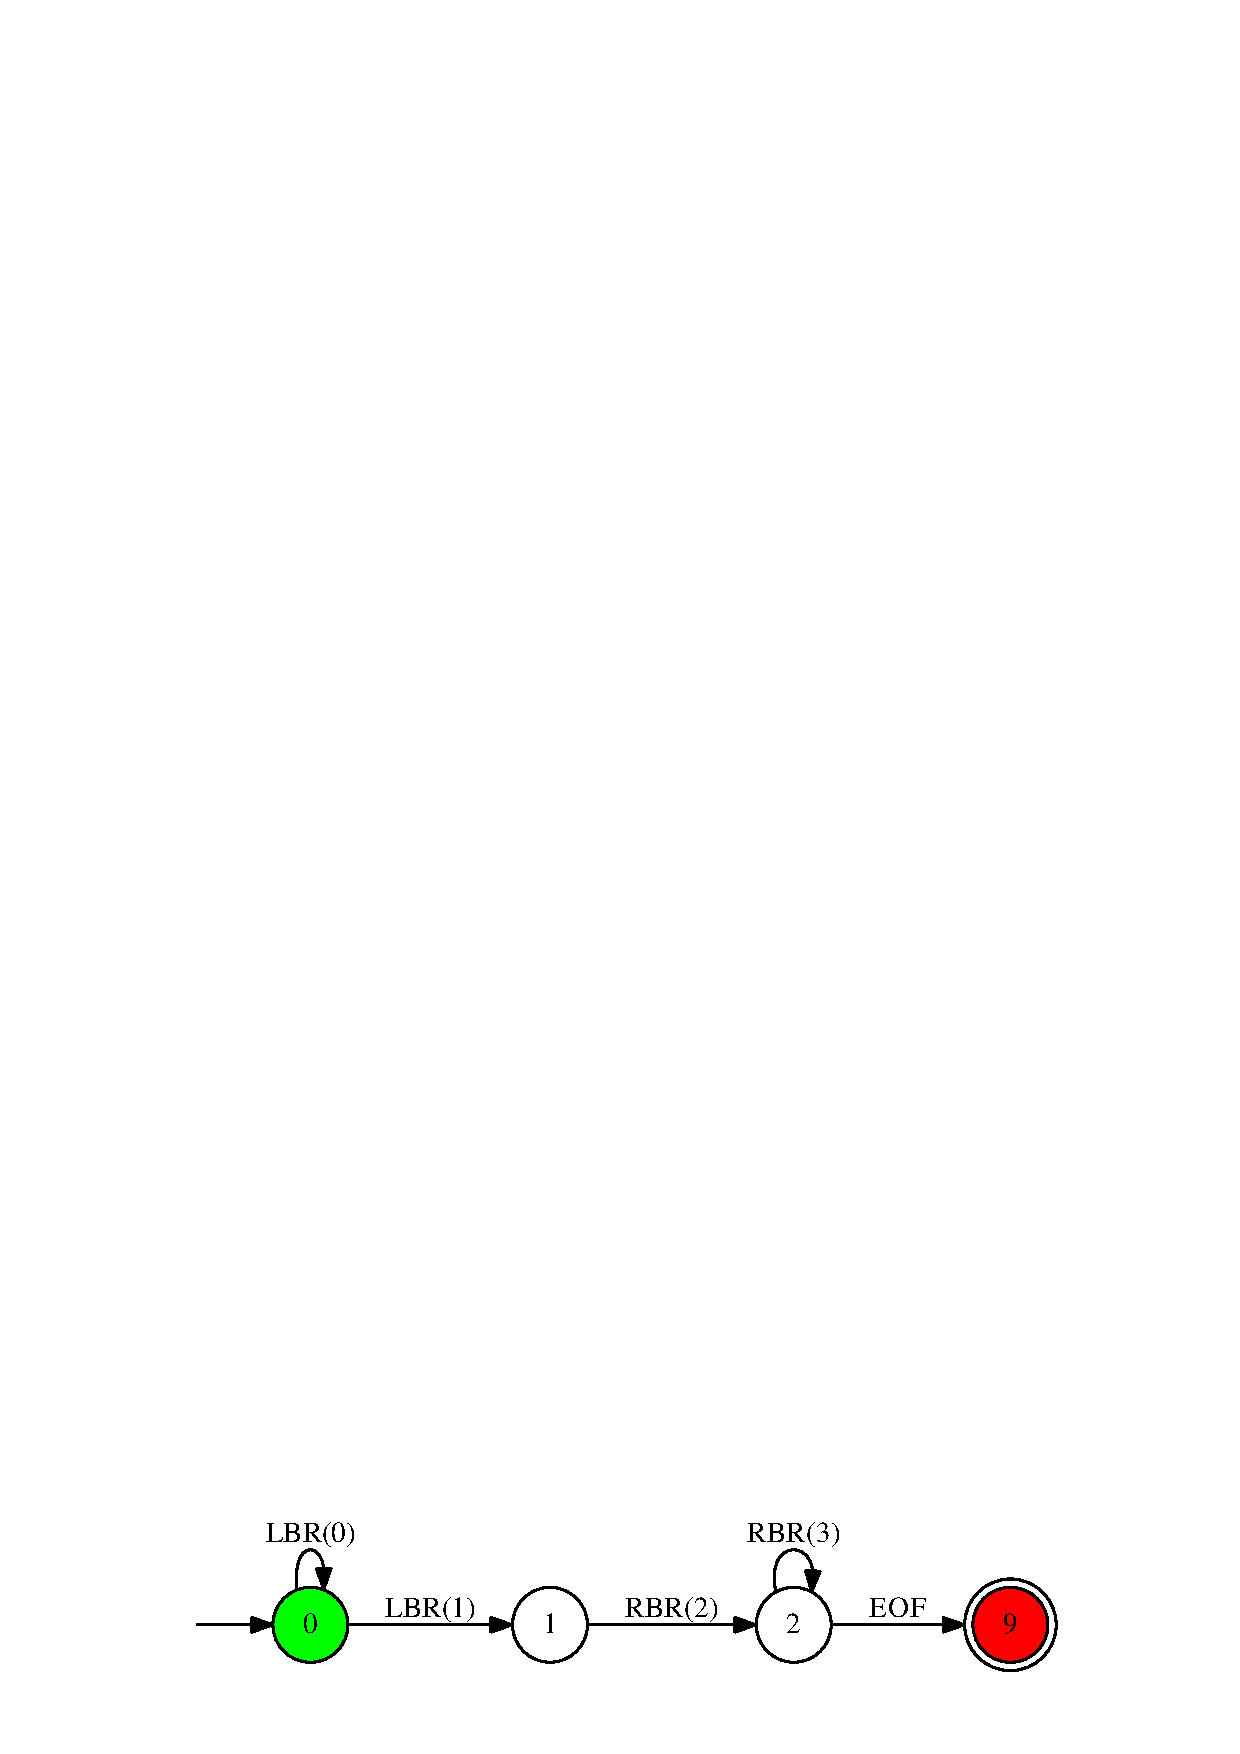
\includegraphics[width=160pt]{pictures/in3.pdf}

    \end{tabular}
\end{center}
\end{frame}


\begin{frame}[t]
    \transwipe[direction=90]
    \frametitle{Пример работы: синтаксический анализ}
%\begin{center}
    \begin{tabular}{p{5.8cm} p{6.2cm}}
\underline{Грамматика:}& \underline{Результат (SPPF):}
\vspace{-20pt}
\\
\vspace{-20pt}

$$
\begin{array}{crcl}
(0)& start\_rule &::=& s \\
(1)& s & ::= & \mbox{\texttt{LBR }} s \mbox{\texttt{ RBR }} s\\
(2)& s & ::= &\varepsilon
\end{array}
$$
&
\\      
\underline{Вход:} \vspace{10pt}&
\\
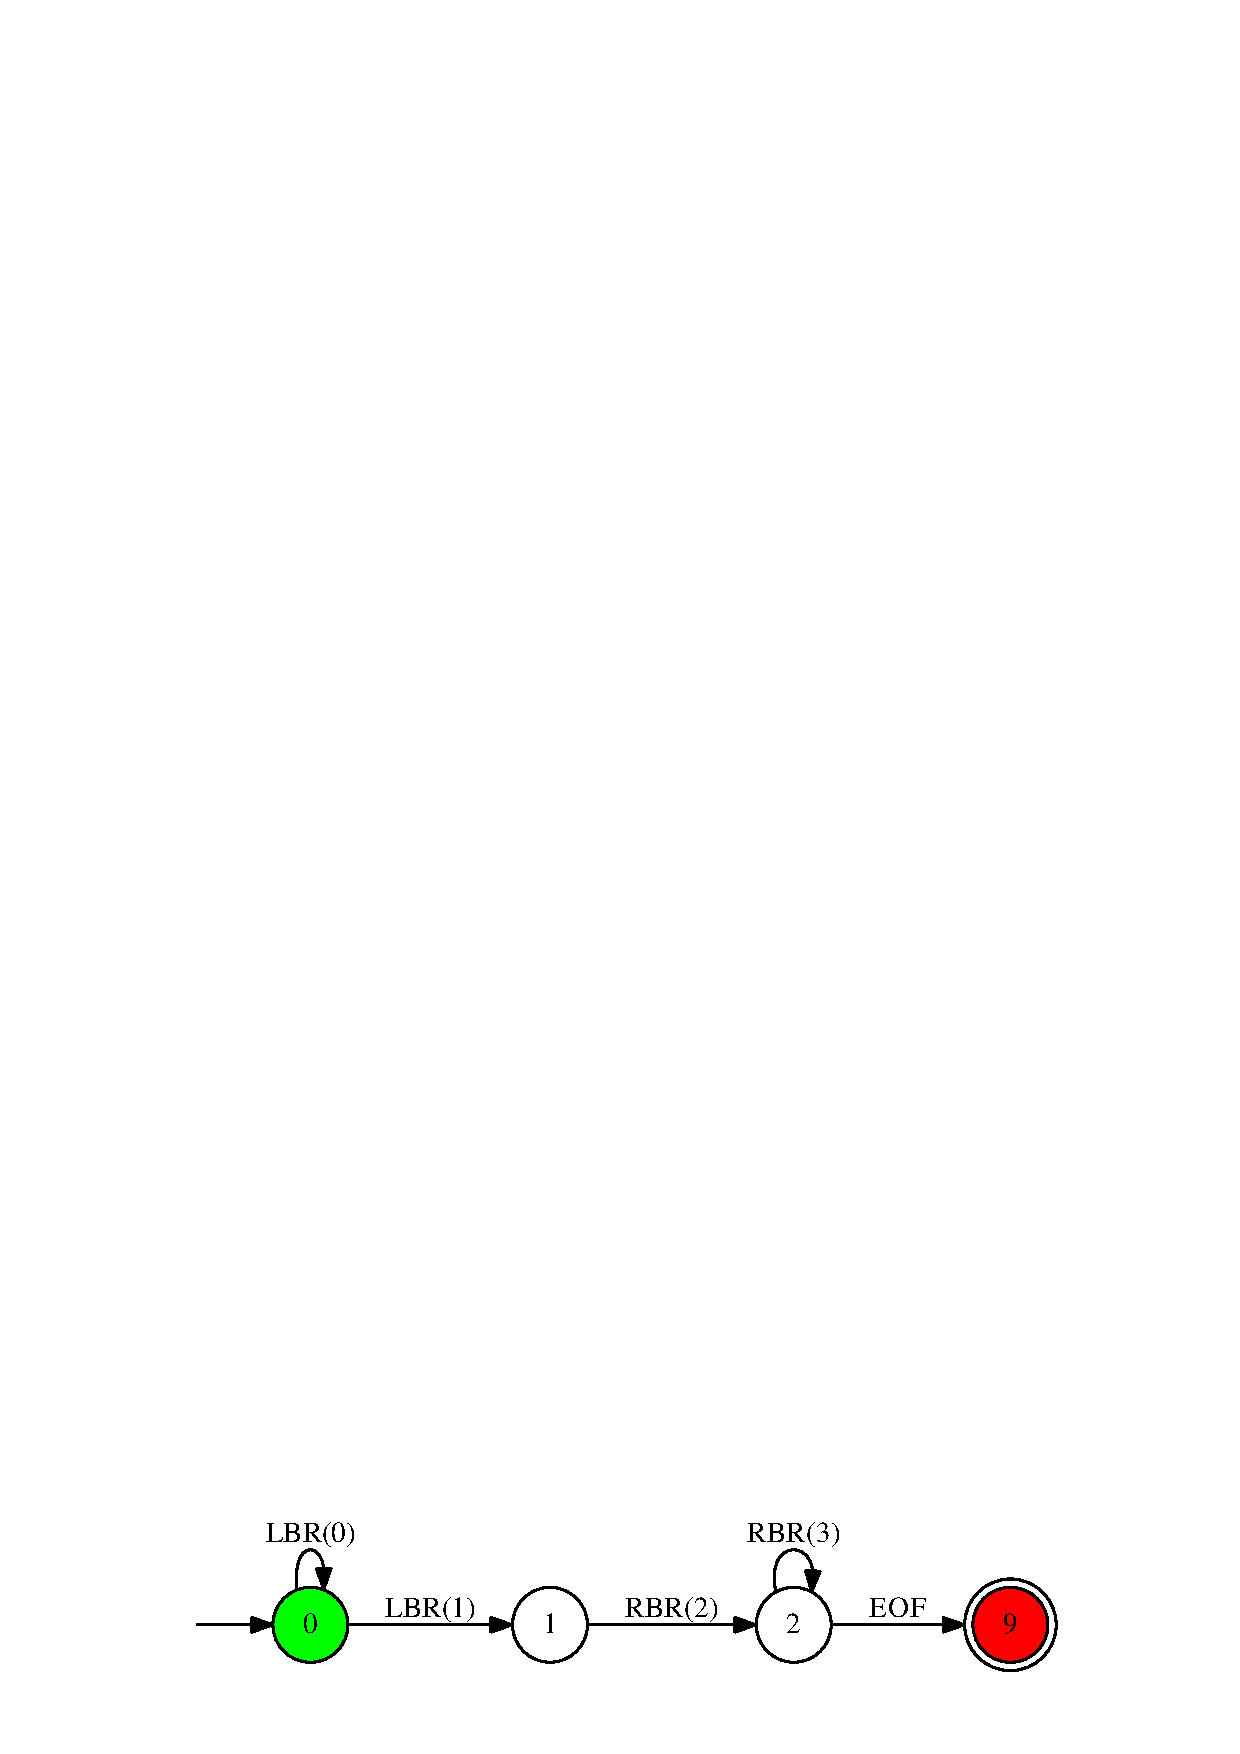
\includegraphics[width=170pt]{pictures/in3.pdf}
& \multirow{-9}*{\!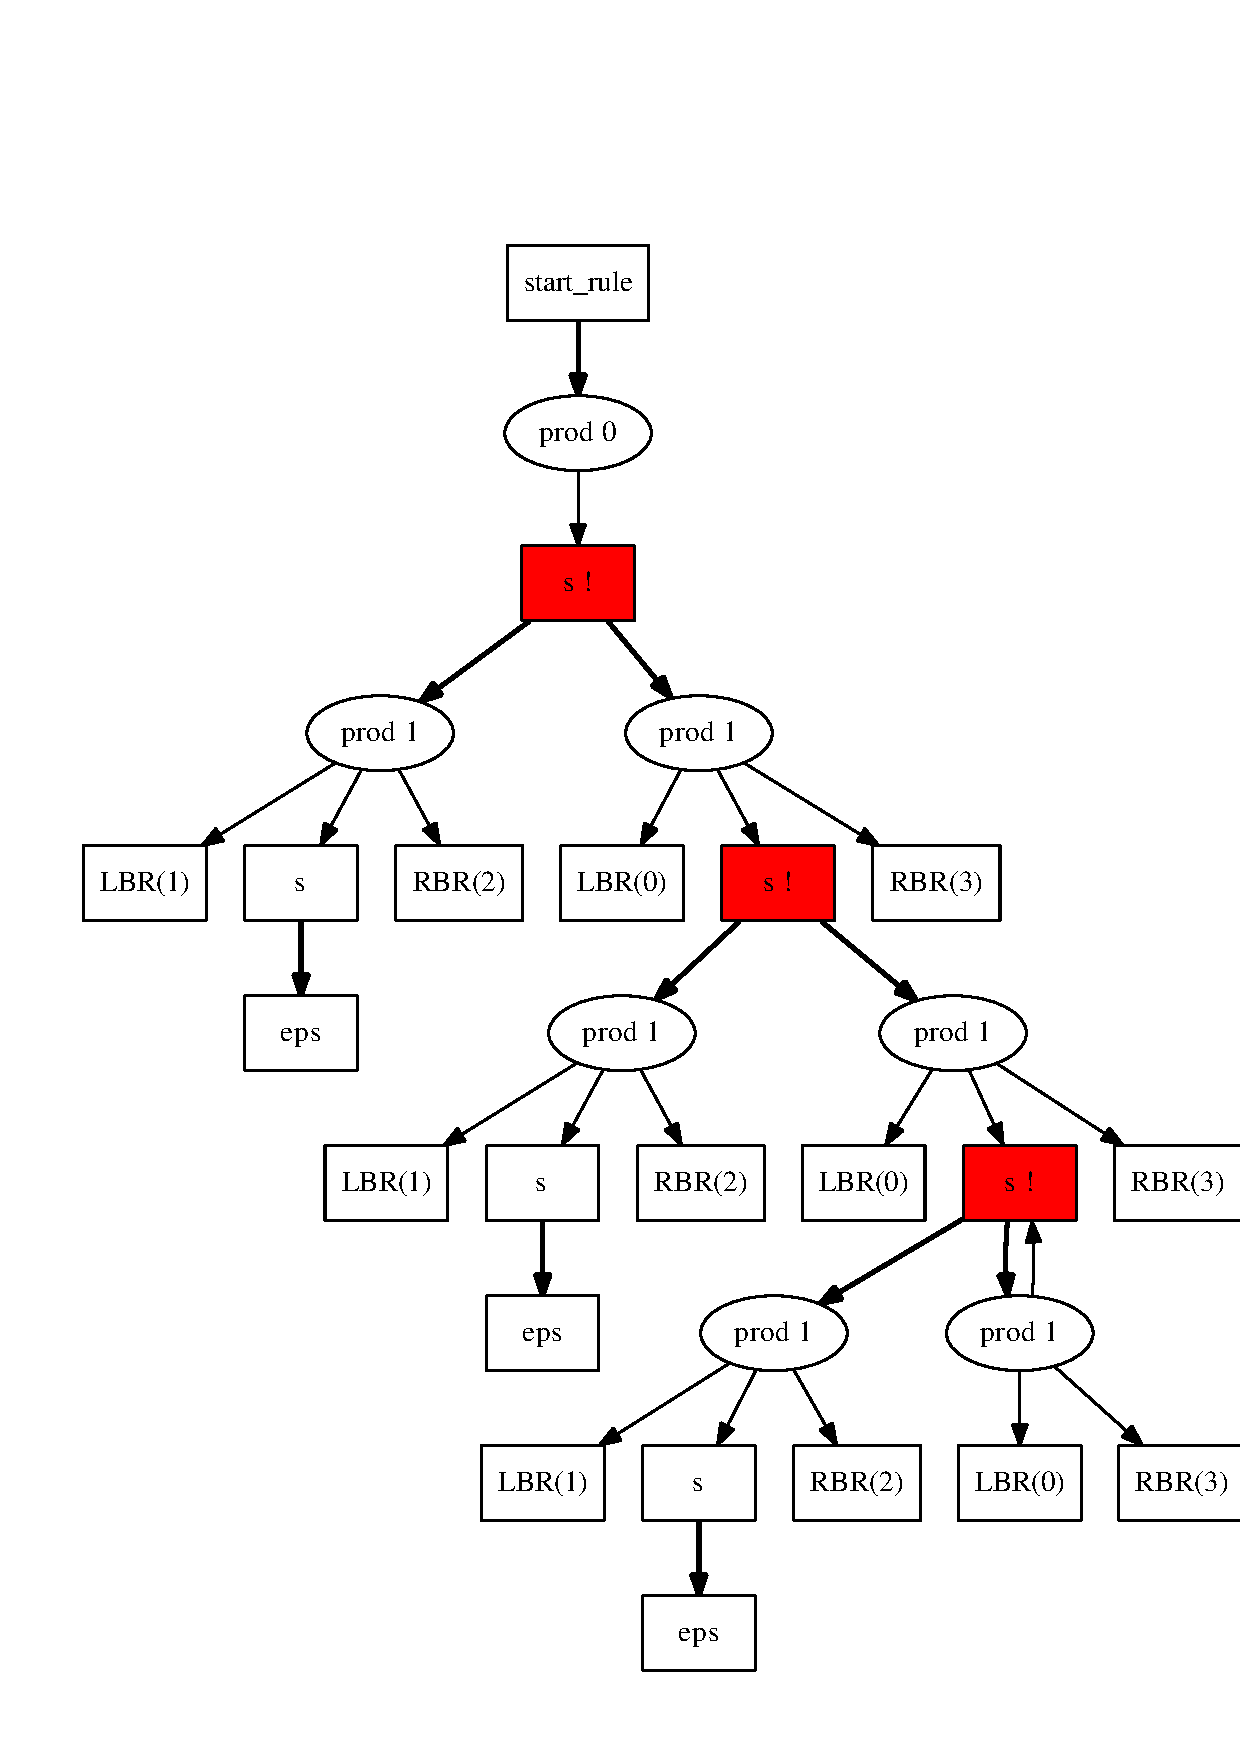
\includegraphics[width=168pt]{pictures/out3.pdf}}
\end{tabular}
%\end{center}

\end{frame}

\begin{frame}
    \transwipe[direction=90]
    \frametitle{Положения, выносимые на защиту}
        \begin{itemize}
            \tikz\node[opacity=0.2,align=left,inner xsep=0pt]
            {%
            \parbox[t]{\linewidth}{%
            \item Алгоритм синтаксического анализа динамически формируемых выражений со 
            следующими свойствами
            \begin{itemize}
                \item обработка произвольной регулярной аппроксимации множества значений выражения 
                \item эффективное управление стеком 
                \item конечность представления леса вывода              
            \end{itemize}
            \item Доказательство завершаемости и корректности предложенного алгоритма
            }%
            };

            \item Архитектура инструментария для разработки программных средств 
            синтаксического анализа динамически формируемых строковых выражений
            \tikz\node[opacity=0.2,align=left,inner xsep=0pt]
            {%
            \parbox[t]{\linewidth}{%
            \item Методика обработки динамически формируемых строковых выражений в контексте реинжиниринга информационных систем  
            }%
            };
        \end{itemize}
\end{frame}
                           
\begin{frame}
    \transwipe[direction=90]
    \frametitle{Архитектура: требования}
    \begin{itemize}
        \item Упростить создание инструментов для анализа динамически формируемых выражений
        \item Предоставить набор готовых компонентов, генератор лексических и синтаксических анализаторов
    \end{itemize}
    \begin{center}
        \includegraphics[width=345pt]{pictures/HighLevelArch.pdf}
    \end{center}
\end{frame}

\begin{frame}
    \transwipe[direction=90]
    \frametitle{Архитектура}
    \includegraphics[width=345pt]{pictures/Components.pdf}
\end{frame}

\begin{frame}
    \transwipe[direction=90]
    \frametitle{Положения, выносимые на защиту}
        \begin{itemize}
            \tikz\node[opacity=0.2,align=left,inner xsep=0pt]
            {%
            \parbox[t]{\linewidth}{%
            \item Алгоритм синтаксического анализа динамически формируемых выражений со 
            следующими свойствами
            \begin{itemize}
                \item обработка произвольной регулярной аппроксимации множества значений выражения 
                \item эффективное управление стеком 
                \item конечность представления леса вывода              
            \end{itemize}
            \item Доказательство завершаемости и корректности предложенного алгоритма
            \item Архитектура инструментария для разработки программных средств 
            синтаксического анализа динамически формируемых строковых выражений
            }%
            };
            \item Методика обработки динамически формируемых строковых выражений в контексте реинжиниринга информационных систем  
        \end{itemize}
\end{frame}


\begin{frame}[t]
    \transwipe[direction=90]
    \frametitle{Метод реинжиниринга встроенного программного кода}
    \begin{center}
        \includegraphics[width=335pt]{pictures/ActivMethodology.pdf}
    \end{center}
\end{frame}

\begin{frame}[t]
    \transwipe[direction=90]
    \frametitle{Ограничения}
    \begin{itemize}
        \item Регулярная аппроксимация
        \begin{itemize}
          \item Встроенный язык может быть минимум контекстно-свободным
          \item Неполнота информации: пользовательский ввод, взаимодействие с подсистемами и т.д.
          \item Потеря точности
        \end{itemize}
        \item Детерминированная КС грамматика для ``эталонного'' языка 
        \item Недостаточная производительность для IDE
        \begin{itemize}
          \item Точность или производительность?
          \item Компоненты заменяемы --- можно найти баланс (так сделано в Alvor)
          \item Оптимизация существующего решения
        \end{itemize}
        \item Работа с SPPF в общем виде плохо изучена
        \begin{itemize}
          \item Какие задачи можно решать над полученным представлением леса разбора?
        \end{itemize}
    \end{itemize}
\end{frame}

\begin{frame}[t]
    \transwipe[direction=90]
    \frametitle{Апробация: трансляция динамического SQL}
    \begin{itemize}
    \item Промышленный проект ЗАО ``Ланит-Терком'' по миграции ИС с MS SQL Server на Oracle Server
    \item 2,7 миллиона строк кода, 2430 точек интереса
        \begin{itemize}
            \item 75\% запросов могли принимать более одного значения
            \item До 212 операторов для формирования выражения, среднее: 40  
        \end{itemize}
    \item 2188 разобрано
    \item 1 не удалось разобрать из-за таймаута
    \item 241 не разобрано из-за неточностей в используемом окружении
  \end{itemize}
  \includegraphics[width=8.5cm]{pictures/dist.png}
\end{frame}

\begin{frame}[t]
    \transwipe[direction=90]
    \frametitle{Апробация: плагин к ReSharper}
        \begin{itemize}
            \item Поддержка встроенных языков в Microsoft Visual Studio IDE
            \begin{itemize}
                \item Подсветка синтаксиса
                \item Подсветка парных скобок
                \item Подсветка ошибок
            \end{itemize}
        \end{itemize}
    \begin{center}
      \includegraphics[width=250pt]{pictures/RShExampe.png}
    \end{center}
\end{frame}

\begin{frame}
    \transwipe[direction=90]
    \frametitle{Публикации (ВАК)}
  \begin{itemize}
      \item Кириленко Я.А., Григорьев С. В., Авдюхин Д. А. Разработка синтаксических анализаторов в проектах по автоматизированному реинжинирингу информационных систем.  Научно-технические ведомости Санкт-Петербургского государственного политехнического университета информатика, телекоммуникации, управление. Т. 3, N 174, 2013. C. 94---98.
      \item Григорьев С. В., Вербицкая Е. А., Полубелова М. И., Иванов А. В., Мавчун Е. В. Инструментальная поддержка встроенных языков в интегрированных средах разработки. Моделирование и анализ информационных систем. Т. 21, N 6, 2014. С. 131---143.
      \item Григорьев С.В., Рагозина А.К. Обобщённый табличный LL-анализ. Системы и средства информатики. Т. 25, N 1, 2015. С. 89---107.
  \end{itemize} 
\end{frame}

\begin{frame}
    \transwipe[direction=90]
    \frametitle{Другие публикации}
  \begin{itemize}
          \item Semen Grigorev, Iakov Kirilenko. GLR-based abstract parsing. In Proceedings of the 9th Central \& Eastern European Software Engineering Conference in Russia (CEE-SECR ’13). 2013. ACM, New York, NY, USA. 1-9 p.
          \item Semen Grigorev, Ekaterina Verbitskaia, Andrei Ivanov, Marina Polubelova, Ekaterina Mavchun. String-embedded language support in integrated development environment. In Proceedings of the 10th Central and Eastern European Software Engineering Conference in Russia (CEE-SECR '14). 2014. ACM, New York, NY, USA. 1-11 p.
          \item Semen Grigorev, Iakov Kirilenko. From Abstract Parsing to Abstract Translation. Proceedings of the Spring/Summer Young Researchers' Colloquium on Software Engineering. 2014. Saint Petersburg, Russia. 1-5 p.
  \end{itemize} 
\end{frame}

\begin{frame}
    \transwipe[direction=90]
    \frametitle{Выступления на конференциях и семинарах}
  \begin{itemize}
          \item CEE-SECR (2012, 2013, 2014)
          \begin{itemize}
              \item Премия Бертрана Мейера за лучшую исследовательскую работу в области программной 
инженерии (2014)
          \end{itemize} 
          \item Parsing@SLE-2013
          \item Семинар по наукоёмкому программному обеспесчению при PSI-2014
          \item Научный семинар по программной инженерии (2013, 2015, СПбПГУ)
          \item SYRCoSE-2014
  \end{itemize} 
\end{frame}


\begin{frame}[fragile] 
    \transwipe[direction=90]
    \frametitle{Алгоритм: псевдокод}
\begin{algorithmic}[1]
\Function{parse}{$grammar, automaton$}
  \State{$inputGraph \gets$ construct inner graph representation of $automaton$}
  \State{$parserSource \gets$ generate RNGLR parser tables for $grammar$}
  \If{$inputGraph$ contains no edges}
    \If{$parserSource$ accepts empty input} {report success}
    \Else { report failure}
    \EndIf
  \Else
    \State{\Call{addVertex}{$inputGraph.startVertex, startState$}}
    \State{$\mathcal{Q}.Enqueue(inputGraph.startVertex)$}
    \While{$\mathcal{Q}$ is not empty}
      \State{$v \gets \mathcal{Q}.Dequeue()$}
      \State{\Call{makeReductions}{$v$}}
      \State{\Call{push}{$v$}}
      \State{\Call{applyPassingReductions}{$v$}}
    \EndWhile
    \If{$v_f.level = q_f$ and $v_f.state$ is accepting} {report success}
    \Else { report failure}
    \EndIf
  \EndIf
\EndFunction
\end{algorithmic}
\end{frame}

\begin{frame}[fragile] 
    \transwipe[direction=90]
    \frametitle{Алгоритм: псевдокод}
\begin{algorithmic}[1]
%\caption{Single vertex processing}
%\label{processVertex}

\Function{makeReductions}{$innerGraphV$}
  \While{$innerGraphV.reductions$ is not empty}
    \State{$(startV, N, l) \gets innerGraphV.reductions.Dequeue()$}
    \State{find the set of vertices $\mathcal{X}$ reachable from $startV$}
    \State{    along the path of length ($l-1$), or $0$ if $l=0$;}
    \State{add $(startV, N, l-i)$ in $v.passingReductions$,}
    \State{    where $v$ is an $i$-th vertex of the path}
    \ForAll{$v_{h}$ in $\mathcal{X}$}
      \State{$state_{t} \gets$ calculate new state by $v_{h}.state$ and nonterminal $N$}
      \State{\Call{addEdge}{$v_{h}, startV, state_{t}, (l=0)$}}
    \EndFor
  \EndWhile
\EndFunction
\end{algorithmic}
\end{frame}


\begin{frame}[fragile] 
    \transwipe[direction=90]
    \frametitle{Алгоритм: псевдокод}
\begin{algorithmic}[1]

\Function{push}{$innerGraphV$}
  \State{$\mathcal{U} \gets$ copy $innerGraphV.unprocessed$}
  \State{clear $innerGraphV.unprocessed$}
  \ForAll{$v_{h}$ in $\mathcal{U}$}  
    \ForAll{$e$ in outgoing edges of $innerGraphV$}
      \State{$push \gets$ calculate next state by $v_{h}.state$ and the token on $e$}
      \State{\Call{addEdge}{$v_{h}, e.Head, push, false$}}
      \State{add $v_{h}$ in $innerGraphV.processed$}
    \EndFor
  \EndFor
\EndFunction

\Function{applyPassingReductions}{$innerGraphV$}
  \ForAll{$(v, edge)$ in $innerGraphV.passingReductionsToHandle$}
    \ForAll{$(startV, N, l) \gets v.passingReductions.Dequeue()$}
      \State{find the set of vertices $\mathcal{X}$,}
      \State{    reachable from $edge$ along the path of length ($l-1$)}
      \ForAll{$v_{h}$ in $\mathcal{X}$}
        \State{$state_{t} \gets$ {\small calculate new state by $v_{h}.state$ and nonterminal $N$}}
        \State{\Call{addEdge}{$v_{h}, startV, state_{t}, false$}}
      \EndFor
    \EndFor
  \EndFor
\EndFunction
\end{algorithmic}
\end{frame}

\begin{frame}[fragile] 
    \transwipe[direction=90]
    \frametitle{Алгоритм: псевдокод}
\begin{algorithmic}[1]
%\caption{GSS construction}
%\label{gss_construction}
\Function{addVertex}{$innerGraphV, state$}
  \State{$v \gets$ find a vertex with state $=state$ in}
  \State{    $innerGraphV.processed \cup innerGraphV.unprocessed$}
  \If{$v$ is not $null$ } \Comment{The vertex have been found in GSS}
    \State{\Return{($v, false$)}} 
  \Else
    \State{$v \gets$ create new vertex for $innerGraphV$ with state $state$}
    \State{add $v$ in $innerGraphV.unprocessed$}
    \ForAll{$e$ in outgoing edges of $innerGraphV$}
      \State{\small calculate the set of zero-reductions by $v$}
      \State{  \small and the token on $e$ and add them in $innerGraphV.reductions$}
    \EndFor
    \State{\Return{$(v, true$)}}
  \EndIf
\EndFunction
\end{algorithmic}
\end{frame}

\begin{frame}[fragile] 
    \transwipe[direction=90]
    \frametitle{Алгоритм: псевдокод}
\begin{algorithmic}[1]
\Function{addEdge}{$v_{h}, innerGraphV, state_{t}, isZeroReduction$}
  \State{$(v_{t}, isNew) \gets$ \Call{addVertex}{$innerGraphV, state_{t}$}}
  \If{GSS does not contain edge from $v_{t}$ to $v_{h}$}
    \State{$edge \gets$ create new edge from $v_{t}$ to $v_{h}$}
    \State{$\mathcal{Q}.Enqueue(innerGraphV)$}
    \If{not $isNew$ and $v_{t}.passingReductions.Count>0$}
      \State{add $(v_{t}, edge)$ in $innerGraphV.passingReductionsToHandle$}
    \EndIf
    \If{not $isZeroReduction$}
      \ForAll{$e$ in outgoing edges of $innerGraphV$}
        \State{{\small calculate the set of reductions by $v$}}
        \State{  {\small{and the token on $e$ and add them in $innerGraphV.reductions$}}}
      \EndFor
    \EndIf
  \EndIf
\EndFunction
\end{algorithmic}
\end{frame}



\end{document}
